\section{Basic Positions on the Cylinder}\label{sec:basic}

\begin{figure*}[!t]
\centering
\begin{subfigure}[t]{0.235\textwidth}\centering
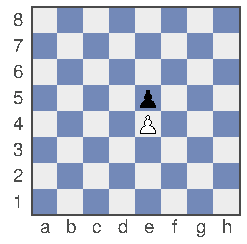
\includegraphics[width=\linewidth]{figures/zero.pdf}
\caption{\pos{W e4 / B e5}: $0$}
\end{subfigure}\hfill
\begin{subfigure}[t]{0.235\textwidth}\centering
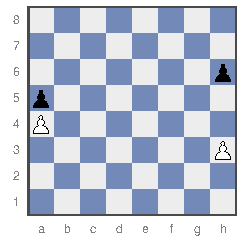
\includegraphics[width=\linewidth]{figures/zero_seam.pdf}
\caption{\pos{W a4 h3 / B a5 h6}: $0$}
\end{subfigure}\hfill
\begin{subfigure}[t]{0.235\textwidth}\centering
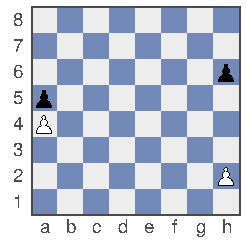
\includegraphics[width=\linewidth]{figures/one.pdf}
\caption{\pos{W a4 h2 / B a5 h6}: $1$}
\end{subfigure}\hfill
\begin{subfigure}[t]{0.235\textwidth}\centering
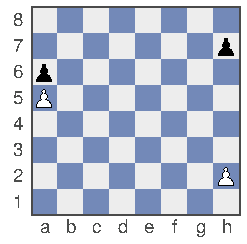
\includegraphics[width=\linewidth]{figures/two.pdf}
\caption{\pos{W a5 h2 / B a6 h7}: $2$}
\end{subfigure}

\medskip
\begin{subfigure}[t]{0.235\textwidth}\centering
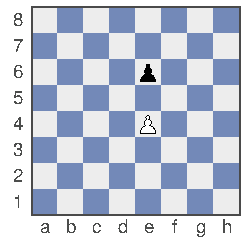
\includegraphics[width=\linewidth]{figures/star.pdf}
\caption{\pos{W e4 / B e6}: $\star$}
\end{subfigure}\hfill
\begin{subfigure}[t]{0.235\textwidth}\centering
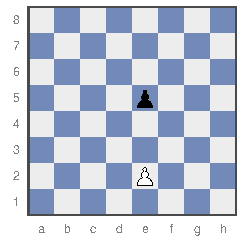
\includegraphics[width=\linewidth]{figures/up.pdf}
\caption{\pos{W e2 / B e5}: ${\uparrow}$}
\end{subfigure}\hfill
\begin{subfigure}[t]{0.235\textwidth}\centering
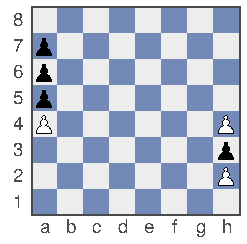
\includegraphics[width=\linewidth]{figures/tiny1_2025.pdf}
\caption{\pos{W a4 h2 h4 / B a5 a6 a7 h3}: $\tinyg{1}$}
\end{subfigure}\hfill
\begin{subfigure}[t]{0.235\textwidth}\centering
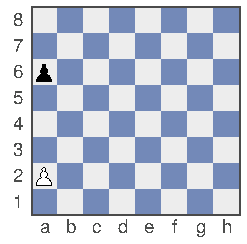
\includegraphics[width=\linewidth]{figures/elkies_dup.pdf}
\caption{\pos{W a2 / B a6}: ${\Uparrow}\star$}
\end{subfigure}
\caption{Basic pawn games. Boards (a)--(g) are cylinders (files a and h adjacent); (h) is drawn on the ordinary
board and has the same value on the cylinder. Each value holds under all three race rules, under both
passed-pawn tests, and with e.p.\ on or off, except (d), which is $2$ only with e.p.\ on and ${\Uparrow}\star$
with e.p.\ off.}
\label{fig:basic}
\end{figure*}

We first build the basic games $0$, $1$, $2$, $\star$, ${\uparrow}$ and Tiny 1 with pawns alone
(Fig.~\ref{fig:basic}); kings join in Section~\ref{sec:kings}. A full discussion of these simple games can be found in \cite{WinningWays}, and their
ordinary-board versions in \cite{Elkies1996,WuYuLandry2020}. Each board in Fig.~\ref{fig:basic} leaves a
file empty, so by Theorem~\ref{thm:cut} it is also a position on an ordinary board: these are Elkies' values,
and the cylinder lets four of them be built across the seam. Values that only a cylinder can make need a pawn on every file
(Section~\ref{sec:atlas}). One remark keeps the walk-throughs short. A move that lets the opponent reply with a
passed pawn, or with anything as bad, is reversible and drops out of the canonical form
\cite{WinningWays}: having only losing moves is the same as having no moves at all \cite{WuYuLandry2020}.

\subsection{The Zero Game}
Let's begin with the zero game, a game in which neither player can move: $0=\game{}{}$. Under normal play it is
a second-player win. In Fig.~\ref{fig:basic}(a) the two pawns in the center are stuck, so neither side has a
move, and the value is $0$.

Fig.~\ref{fig:basic}(b) is a zero game that uses the seam. If white goes first, it must play h3--h4, and the
black pawn on a5 captures it across the seam, a5$\times$h4, leaving a passed pawn. If black goes first, h6--h5
is met by a4$\times$h5 in the same way. Whoever moves first loses, so this is again $0$. As in
\cite{WuYuLandry2020}, many zero games are symmetric like this one.

\subsection{The Games \texorpdfstring{$1$}{1} and \texorpdfstring{$2$}{2}}
In Fig.~\ref{fig:basic}(c) the deadlocked pawns on a4 and a5 stay, but the white h-pawn starts one square
further back. White can play h2--h3, which leaves the zero game of Fig.~\ref{fig:basic}(b); the double step
h2--h4 only loses the pawn to a5$\times$h4. Black has one move, h6--h5, and a4$\times$h5 gives white a passed
pawn. Thus $G=\game{0}{}=1$, the one game.

In Fig.~\ref{fig:basic}(d) the a-pawns stand one rank higher, and the white h-pawn has two squares to cross.
White can play h2--h4, which leaves the zero game (b) moved up one rank, or h2--h3, which leaves the one game
(c) moved up one rank. Black has only losing moves: h7--h6 is met by a5$\times$h6, and the double step h7--h5 by
a5$\times$h6 en passant across the seam. Thus $G=\game{0,1}{}=2$, the two game. This value needs en passant:
with e.p.\ off, h7--h5 is safe and the value falls to ${\Uparrow}\star$. To get $-1$ or $-2$, switch the black and
white pawns and turn the board through $180^\circ$ \cite{WuYuLandry2020}.

\subsection{The Infinitesimals \texorpdfstring{$\star$, ${\uparrow}$}{Star, Up} and Tiny 1}
The first infinitesimal is star, in which both white and black can move to the zero game:
$\star=\game{0}{0}$. In Fig.~\ref{fig:basic}(e), e4--e5 and e6--e5 each lock the file, so $G=\star$, a
first-player win.

The formal definition of up is ${\uparrow}=\game{0}{\star}$. In Fig.~\ref{fig:basic}(f), white can play e2--e3,
which leaves star, or e2--e4, which locks the file and leaves $0$. Black can only play e5--e4, which leaves
star. Thus $G=\game{0,\star}{\star}$. Star is a reversible move for white: black answers e2--e3 with e5--e4 and
reaches $0$, and since white wins $G$ when black starts ($G\ge 0$), this reply is at least as good for black as
the position before white's move. So $G=\game{0}{\star}={\uparrow}$. Up is positive, so white wins whoever
starts, yet it is smaller than every positive number. Switching the colors as above gives ${\downarrow}$.

Tiny 1 is defined as $\tinyg{1}=\ggame{0}{0\mid -1}$. In Fig.~\ref{fig:basic}(g), white can take the black
pawn across the seam, h4$\times$a5, which leaves every pawn blocked: $0$. White can also advance h4--h5, but
black answers a6$\times$h5 and wins, so this move drops out. Black can only take white's pawn, a5$\times$h4.
From there white can lock the a-file with a4--a5, leaving $0$, while black can play a6--a5 and keep the spare
move a7--a6, leaving $-1$. So black's capture leads to $\game{0}{-1}=-\tfrac12\pm\tfrac12$, and
$G=\ggame{0}{0\mid -1}=\tinyg{1}$, a positive infinitesimal.

A single file can hold more than one might expect. In Fig.~\ref{fig:basic}(h), white can play a2--a3, leaving
$0$ (each side's move from there leaves star), or a2--a4, leaving $\star$. Black can only play a6--a5, which
leaves the up position of Fig.~\ref{fig:basic}(f) on the a-file. So $G=\game{0,\star}{{\uparrow}}$. Just as in
(f), star is reversible for white, so $G=\game{0}{{\uparrow}}={\Uparrow}\star$, ``double-up star'', one of Elkies'
examples \cite{Elkies1996}.
